\documentclass{article}
\usepackage{tikz}
\usetikzlibrary{decorations.markings}
\pagestyle{empty}
\begin{document}
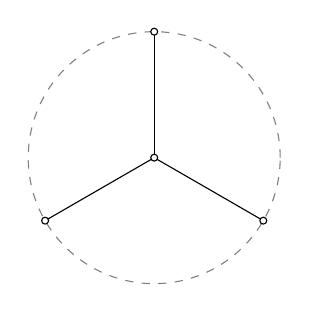
\begin{tikzpicture}
[scale=1.6,every node/.style={draw, circle, fill=white, inner sep=0pt, outer sep=0pt, minimum size=2.5pt},
->-/.style={decoration={markings, mark=at position .5 with{\arrow{>}}}, postaction={decorate}},
-<-/.style={decoration={markings, mark=at position .5 with{\arrow{<}}}, postaction={decorate}}]
\draw[gray, dashed] (0,0) circle (1.0);
 \node (2) at (0.0,1.0) {};
\node (3) at (-0.866025,-0.5) {};
\node (4) at (0.866025,-0.5) {};
\node (1) at (0.0,0.0) {};
\draw[out=149.999988, in=330.0] (4) to (1);
\draw[out=30.000012, in=210.0] (3) to (1);
\draw[out=-90.0, in=90.0] (2) to (1);
\end{tikzpicture}
\end{document}